\documentclass{standalone}
\usepackage{ tikz }
\usetikzlibrary{shapes}
\usetikzlibrary{plotmarks}
\usepackage{ xparse }
\usepackage{../../../macros}

\begin{document}
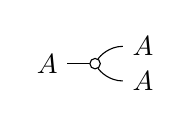
\begin{tikzpicture}[yscale=-1,x=1em,y=1.25em]
    \node [anchor=east] at (-1,0) {$A$};
    \draw (-1,0) -- (0,0);
    \node (C1) [draw, circle, fill=white, scale=0.4] at (0,0) {};
    \node (A1) [anchor=west] at (1,-0.5) {$A$};
    \node (A2) [anchor=west] at (1,0.5) {$A$};
    \draw (C1) to[out=285, in=180] (A1);
    \draw (C1) to[out=75, in=180] (A2);
\end{tikzpicture}
\end{document}